\documentclass[./\jobname.tex]{subfiles}
\begin{document}

\section{Multimodality and Symmetry}
\label{chap:multimodality_and_symmetry}

The optimisation algorithm tries to find the best approximation of $N$ kernels to the solution of a differential equation. Assume, that a kernel $K$ is fully defined by a vector of parameters $\mathbf{p}$. The best fit is defined as 

\begin{equation}
\mathbf{\hat{p}_{apx}} = \left[\underbrace{\left[ \mathbf{\hat{p}}_{K_0} \right] }_{\text{kernel 0}}, \cdots \underbrace{\left[ \mathbf{\hat{p}}_{K_i} \right] }_{\text{kernel i}}, \cdots \underbrace{\left[ \mathbf{\hat{p}}_{K_N} \right]}_{\text{kernel N}} \right]^T
\end{equation}

where the parameters $\mathbf{\hat{p}}$ of every kernel are chosen optimally. The optimal kernel functions $K(\mathbf{\hat{p}}_{K_i}, \mathbf{x})$ are summed up to form the optimal approximation $\hat{u}_{apx}(\mathbf{x})$. 

\begin{equation}
\label{eq:uapx_kernel_sum}
\hat{u}_{apx}(\mathbf{x}) = \sum_{i=0}^{N} K(\mathbf{\hat{p}}_{K_i}, \mathbf{x})
\end{equation}

Since the order of the summation is irrelevant, any kernel-wise permutation describes an optimal solution $\mathbf{\hat{p}_{apx}}$. Thus, the fitness function $F(u_{apx}(\mathbf{x}))$ has at least $N!$ number of local optima. 

Further, a symmetry in the location of the optima is observed. All optima lay on the surface of the hypersphere that is centred at the origin and has a radius of $r = || \mathbf{\hat{p}_{apx}} ||$. 

The following 3D plot in figure \ref{fig:optima_distribution} shows an exemplary distribution of optima on the fitness function. For the sake of simplicity, a kernel now consists of only one parameter. As an example, the vector $\mathbf{\hat{p}_{apx}} = \left[ 2, 1, -1 \right]^T$ describes an optimal solution that consists of 3 kernels. Any permutation of these three coordinates is itself a perfect fit. 

\begin{figure}[H]
	\centering
	\noindent\adjustbox{max width=0.7\linewidth}{
		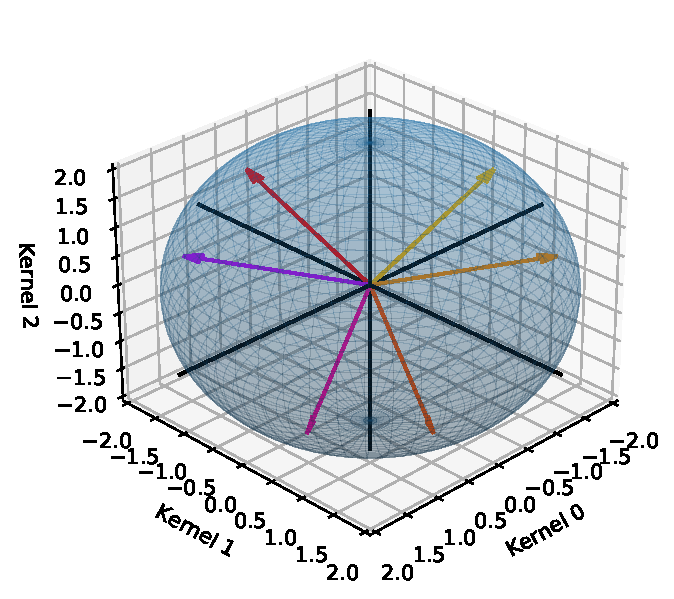
\includegraphics[width=\textwidth]{../img/pdf/symmetry.pdf}
	}
	\unterschrift{Distribution of exemplary optima on the fitness function in 3D space.}{}{}
	\label{fig:optima_distribution}
\end{figure}

This symmetry is independent of the kernel type. Large parts of the fitness function, such as the weighting and penalty factors or the number of collocation points, have no influence on the actual radial arrangement of the optima. 



\end{document}